La obtención de la forma aparente de los Radios Característicos de los choques de Proa
no se obtiene de manera analítica de forma sencilla, por lo que recurrimos a hacer
aproximaciones a la forma de un choque dado, utilizando las cuádricas de revolución.
Éstas cuádricas dan un buen ajuste pero no son capaces de reproducir la forma completa
de un choque de proa dado, por lo que recurrimos al uso de dos cuádricas que en conjunto
ajustan a la forma completa del choque: una para la ``cabeza'' del choque, y otro para la cola.
Y cómo ya vimos en la sección , los radios característicos aparentes se pueden obtener de
manera sencilla para estas superficies.

\begin{figure*}
  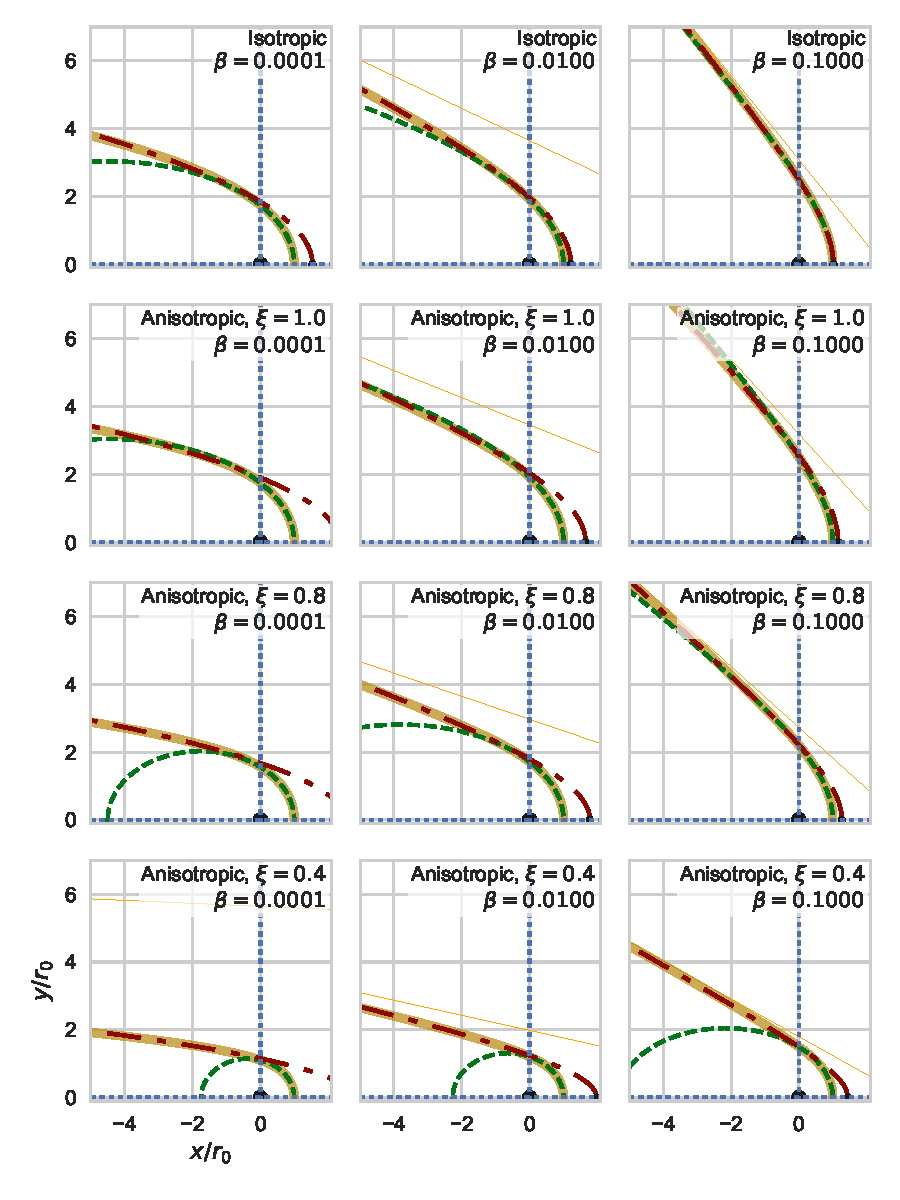
\includegraphics[width = 0.8\linewidth]{conic-head-tail-analytic}
  \label{fig:conic-head-tail-fit}
  \caption{Ajuste de dos cuádricas a las soluciones de capa delgada. La línea gruesa continua
    representa la forma de un choque bajo la aproximación de capa delgada (capítulo
    \ref{chap:hipersonica}) para los parámetros enlistados en cada pánel. La línea verde es el
    ajuste obtenido para la cabeza, mientras que la roja corresponde al ajuste para la cola.}
\end{figure*}


\section{Ajustes a la cabeza}

Utilizando las ecuación (\ref{eq:thc2})  de la sección \ref{sec:conic-char-radii} y las ecuaciones
(\ref{eq:CRW-Rc}) y (\ref{eq:CRW-R90}) de la sección \ref{sec:CRW-2-winds} podemos calcular el parámetro
$\theta_c$ que nos indicará el tipo de cónica que ajusta mejor a cada solución del modelo de capa delgada
en función de los parámetros $\beta$ y $\xi$: 

 \begin{align}
   \tan\theta_c = \left|\frac{3\xi\left(1 + \beta^{1/2}\right)^2}{\left(1 - \xi\beta\right)^2
   \left(1 + \frac{1}{5}\xi\beta\right)} - \frac{2}{\left|1 - 2\gamma\right|}\right|^{1/2}
 \end{align}

 En la figura  se ilustra la dependencia de $\theta_c$ con los parámetros $\beta$ y $\xi$, así como al tipo de
 cónica que ajusta mejor tanto la cabeza como la cola de cada solución a la forma de los choques de proa.
 
 \section{Ajustes a la cola}

 En el caso general del problema de capa delgada, el comportamiento de la cola tiende a ser hiperbólico, dado que
 el ángulo polar $\theta$ tiende a un valor asintótico denominado como $\theta_\infty$. Este ángulo es tal que
 $\theta_\infty + \theta_{1\infty} = \pi$ y se calcula resolviendo la siguiente ecuación explícita:

 \begin{align}
   
 \end{align}

 El ajuste a la hipérbola se logra ajustando tres parámetros fundamentales: $\theta_c = \theta_\infty - \pi$,
 la distancia entre la hipérbola y el centro de ésta a lo largo del eje focal $a_t$ y la distancia entre el origen
 y el centro de la hipérbola $x_{0,t}$. $a_t$ y $x_{0,t}$ se obtienen inicialmente con un ajuste numérico para una
 malla de valores de $\beta$ y $\xi$. Posteriormente hacemos tres ajustes anidados en tres niveles para determinar
 de manera analítica los parámetros de la hipérbola en función de $\beta$ y $\xi$. A continuación mostramos las
 funciones y los parámetros que mejor ajustan a la cola para cada solución a la forma de los choques de proa:

 \begin{align}
   x_{0,t} = 0.7\beta^{-0.55}\left[C_3\left(\log_{10}\beta\right)^3 + C_2\left(\log_{10}\beta\right)^2 +
   C_1\left(\log_{10}\beta\right) + C_0\right] \label{eq:tail-analytic-x0}\\
   (x_{0,t} - a_t) = D_2\left(\log_{10}\beta\right)^2 + D_1\left(\log_{10}\beta\right) + D_0
   \label{eq:tail-analytic-x0-minus-a}
 \end{align}

 Donde:
 
 \begin{alignat}{2}
   \label{eq:tail-analytic-coeffs-c}
   C_k &= c_{2,k}\xi^2 + c_{1,k}\xi + c_{0,k} & \mathrm{para~}k=[0,1,2,3] \\
   \label{eq:tail-analytic-coeffs-d}
   D_k &= d_{2,k}\xi^2 + d_{1,k}\xi + d_{0,k} & \mathrm{para~}k=[0,1,2]
 \end{alignat}

 Los coeficientes de los ajustes para la cola se muestran en la tabla \ref{tab:tail-fit-coeffs}:


\newcommand\iso{\ensuremath{^{\mathrm{iso}}}}

\begin{table}
  \caption{Coeficientes del ajuste hiperbólico a la cola de los choques de Proa}
  \label{tab:tail-fit-coeffs}
  \renewcommand\arraystretch{1.2}
  \setlength\tabcolsep{0.5\tabcolsep}
  \begin{tabular}{@{}llll@{}}
    \toprule
    Ecuación~(\ref{eq:tail-analytic-x0}) & 
    \multicolumn{3}{l}{
    Ecuación~(\ref{eq:tail-analytic-coeffs-c}) \dotfill
    } \\ \midrule
    \( C\iso_0 = +1.3195     \)    
    & \( c_{0,0} = +2.0758   \)  
    & \( c_{1,0} = -0.2309   \)  
    & \( c_{2,0} = -0.2532   \)\\
      \( C\iso_1 = +0.4229     \)    
    & \( c_{0,1} = +0.9571   \)  
    & \( c_{1,1} = -0.1530   \)  
    & \( c_{2,1} = -0.2487   \)\\
      \( C\iso_2 = +0.1092     \)    
    & \( c_{0,2} = +0.2528   \)  
    & \( c_{1,2} = -0.0360   \)  
    & \( c_{2,2} = -0.0794   \)\\
      \( C\iso_3 = +0.0051     \)    
    & \( c_{0,3} = +0.0171   \)  
    & \( c_{1,3} = -0.0010   \)  
    & \( c_{2,3} = -0.0095   \)\\ \midrule
    Ecuación~(\ref{eq:tail-analytic-x0-minus-a}) &
    \multicolumn{3}{l}{
    Ecuación~(\ref{eq:tail-analytic-coeffs-d}) \dotfill
    } \\ \midrule
    \( D\iso_0 = +0.7962   \)    
    & \( d_{0,0} = +0.8516 \)  
    & \( d_{1,0} = -0.0907 \)  
    & \( d_{2,0} = -0.2002 \)\\
      \( D\iso_1 = -0.2363   \)    
    & \( d_{0,1} = -0.7620 \)  
    & \( d_{1,1} = +0.1411 \)  
    & \( d_{2,1} = -0.0295 \)\\
      \( D\iso_2 = -0.0126   \)    
    & \( d_{0,2} = -0.0683 \)  
    & \( d_{1,2} = +0.0390 \)  
    & \( d_{2,2} = -0.0236 \)\\
    \bottomrule
  \end{tabular}
\end{table}

 
 En el apéndice  se muestran los detalles de cómo se obtuvieron los coeficientes de la tabla \ref{tab:tail-fit-coeffs}.
 
 \subsection{Ajustes a la cabeza y la cola en el caso de la interacción con un viento plano--paralelo}

 \section{Proyección en el plano del cielo para el modelo de capa delgada}

 
 